\section{The MSL Radiation Assessment Detector}
\label{sec:mslrad}

Built in a cooperation between the University of Kiel and Southwest Research Institute, the \acl{RAD}\acused{RAD} \citep[\acs{RAD},][]{Hassler-2012-MSLRAD} instrument onboard the \acl{MSL}\acused{MSL} \citep[\acs{MSL},][]{Grotzinger-2012} mission provided the first-ever direct radiation measurements on the surface of Mars. It is designed to measure both charged and neutral particles, and calculate particle spectra as well as dosimetric quantities, such as the \ac{TID} rate and \ac{LET} spectra. This aligns with its main science objectives, which include the characterization of energetic particle spectra on the surface of Mars (\acp{GCR} and \acp{SEP}) and the determination of the radiation hazard for past or present life on Mars or for future human Mars missions. Consequently, \ac{RAD} not only been continuously measuring the radiation environment on the Martian surface since the \textit{Curiosity} rover's landing on August 6, 2012, but has also been active during the most part of its 9-month flight to Mars (the so-called cruise phase) to evaluate the radiation dose that astronauts would receive when traveling to Mars.

\begin{figure}
	\centering
	\includegraphics[width=0.4\linewidth]{images/rad}
	\caption[Photo of the \acs{RAD} sensor head]{A photo of the \ac{RAD} sensor head before it was mounted on the \ac{MSL} spacecraft. The red protection cap was removed after installation on the rover. Source: NASA/JPL-Caltech/SwRI}
	\label{fig:rad-photo}
\end{figure}

The \ac{RAD} sensor head (shown in \autoref{fig:rad-photo}) is mounted on the top deck of the rover, pointing towards the zenith. It is composed of three hexagonal silicon solid-state detectors (A, B, and C) with a thickness of \SI{300}{\micro\meter} each, mounted in a stack to form a charged particle telescope (\autoref{fig:rad-sensorhead}) with an opening angle of about \SI{60}{\degree}. Each detector is divided into an inner and an outer segment.
Directly below the charged particle telescope follows the D detector, a cesium iodide (CsI) scintillator in the shape of a truncated hexagonal pyramid. Its shape is chosen so that it aligns with the inner segment of C and follows the opening angle of the charged particle telescope (shown with dashed lines in \autoref{fig:rad-sensorhead}). The E detector, which is located below D, is a plastic scintillator and mainly responsible for neutral particle detection. D and E are surrounded by another plastic scintillator (F), which is used as an anticoincidence shield to reject ions that enter D or E from the sides.

\begin{figure}
	\centering
	%\documentclass{standalone}
%\usepackage{tikz}
%\usepackage{amsmath}

%\usetikzlibrary{calc}
%\usetikzlibrary{decorations.pathmorphing}

%\definecolor{light-gray}{gray}{0.9}

%\begin{document}
\begin{tikzpicture}[scale=0.8]
    \tikzset{%
        add/.style args={#1 and #2}{
            to path={%
                ($(\tikztostart)!-#1!(\tikztotarget)$)--($(\tikztotarget)!-#2!(\tikztostart)$)%
                \tikztonodes},add/.default={.2 and .2}}
    }  
    
    \def\bottomwidth{3.25}
    \def\midwidth{1.8}
    \def\topwidth{1.65}
    \def\bottomheight{2.5}
    \def\midheight{4.375}
    \def\Fthickness{1}
    \def\Sithickness{0.1}
    \def\BCdistance{0.15}
    \def\topheight{8.375}
    
    % FOV
    \draw[add=0 and 0.3, dashed] (\midwidth - \Fthickness, \midheight) to (-\topwidth, \topheight);
    \draw[add=0 and 0.3, dashed] (-\midwidth + \Fthickness, \midheight) to (\topwidth, \topheight);
    
    \draw[|<->|] (-\topwidth, \topheight) ++ (90+30:0.5) arc (90+30:90-30:{\topheight-\midheight-0.2}) node[pos=0.4, above] {\small\SI{60}{\degree}};

    % A
    \draw[fill=light-gray] (-\topwidth, \topheight - \Sithickness) rectangle (\topwidth, \topheight);
    \draw (-\midwidth + \Fthickness, \topheight - \Sithickness) --  (-\midwidth + \Fthickness, \topheight);
    \draw (-\midwidth + \Fthickness, \topheight - \Sithickness) --  (-\midwidth + \Fthickness, \topheight);
    \draw (\midwidth - \Fthickness, \topheight - \Sithickness) --  (\midwidth - \Fthickness, \topheight);
    \draw (\midwidth - \Fthickness, \topheight - \Sithickness) --  (\midwidth - \Fthickness, \topheight);
    \draw[latex-] (-\topwidth, \topheight - \Sithickness / 2) -- (-\topwidth - 0.5, \topheight - \Sithickness / 2) node[left] {A};
    
    % B
    \draw[fill=light-gray] (-\topwidth, \midheight + \BCdistance) rectangle (\topwidth, \midheight + \BCdistance + \Sithickness);
    \draw (-\midwidth + \Fthickness, \midheight + \BCdistance) --  (-\midwidth + \Fthickness, \midheight + \BCdistance + \Sithickness);
    \draw (-\midwidth + \Fthickness, \midheight + \BCdistance) --  (-\midwidth + \Fthickness, \midheight + \BCdistance + \Sithickness);
    \draw (\midwidth - \Fthickness, \midheight + \BCdistance) --  (\midwidth - \Fthickness, \midheight + \BCdistance + \Sithickness);
    \draw (\midwidth - \Fthickness, \midheight + \BCdistance) --  (\midwidth - \Fthickness, \midheight + \BCdistance + \Sithickness);
    \draw[latex-] (-\topwidth, \midheight + \BCdistance + \Sithickness / 2) -- (-\topwidth - 0.5, \midheight + \BCdistance + \Sithickness / 2 + 0.3) node[left] {B};
    
    % C
    \draw[fill=light-gray] (-\topwidth, \midheight) rectangle (\topwidth, \midheight + \Sithickness);
    \draw (-\midwidth + \Fthickness, \midheight) --  (-\midwidth + \Fthickness, \midheight + \Sithickness);
    \draw (-\midwidth + \Fthickness, \midheight) --  (-\midwidth + \Fthickness, \midheight + \Sithickness);
    \draw (\midwidth - \Fthickness, \midheight) --  (\midwidth - \Fthickness, \midheight + \Sithickness);
    \draw (\midwidth - \Fthickness, \midheight) --  (\midwidth - \Fthickness, \midheight + \Sithickness);
    \draw[latex-] (-\topwidth, \midheight + \Sithickness / 2) -- (-\topwidth - 0.5, \midheight + \Sithickness / 2) node[left] {C};
    
    % border of ABC
    \draw (-\topwidth, \midheight) -- (-\topwidth, \topheight);
    \draw (\topwidth, \midheight) -- (\topwidth, \topheight);
    
    % D
    \draw[fill=light-gray] (\bottomwidth - \Fthickness, \bottomheight) --  (-\bottomwidth + \Fthickness, \bottomheight) -- (-\midwidth + \Fthickness, \midheight) -- (\midwidth - \Fthickness, \midheight) -- (\bottomwidth - \Fthickness, \bottomheight);   
    \node at (0, {\bottomheight + (\midheight - \bottomheight) / 2}) {D};   
    
    % E
    \draw[fill=green!50] (\bottomwidth - \Fthickness, \bottomheight) -- (\bottomwidth - \Fthickness, \Fthickness) --
    (-\bottomwidth + \Fthickness, \Fthickness) --  (-\bottomwidth + \Fthickness, \bottomheight) -- (\bottomwidth - \Fthickness, \bottomheight);  
    \node at (0, {\Fthickness + (\bottomheight - \Fthickness) * 0.4}) {E};   
    
    % F
    \draw[fill=Dandelion!50] (-\bottomwidth, 0) -- (\bottomwidth, 0) -- (\bottomwidth, \bottomheight) -- (\midwidth, \midheight) --
    (\midwidth - \Fthickness, \midheight) -- (\bottomwidth - \Fthickness, \bottomheight) -- (\bottomwidth - \Fthickness, \Fthickness) --
    (-\bottomwidth + \Fthickness, \Fthickness) --  (-\bottomwidth + \Fthickness, \bottomheight) -- (-\midwidth + \Fthickness, \midheight) --
    (-\midwidth, \midheight) -- (-\bottomwidth, \bottomheight) -- (-\bottomwidth, 0);     
    \node at (0, \Fthickness / 2) {F};
    
    % trajectories of ions
    \draw[thick, green, -latex] (-\topwidth*0.7, \topheight*1.25) node[above, align=center] {\small Ion\\ \small (accepted)}
     -- ({-(\midwidth - \Fthickness) * 0.5}, \midheight + \Sithickness / 2);
    \draw[thick, green, -latex] (\topwidth*0.65, \topheight*1.25) node[above, align=center] {\small Ion\\ \small (accepted)}
     -- ({-(\midwidth - \Fthickness) * 0.5}, {\bottomheight +  (\midheight - \bottomheight) / 2});
    \draw[thick, red, -latex] (0, \topheight*1.4) node[above, align=center] {\small Ion\\ \small (rejected)}
     -- (0, \topheight - \Sithickness / 2);
    \draw[thick, red, -latex] (\bottomwidth, \midheight) node[above right, align=center] {\small Ion\\ \small (rejected)}
    -- (\bottomwidth * 0.4, {\bottomheight + (\midheight - \bottomheight) * 0.2});
    
    % trajectory of neutron
    \draw[thick, gray, -latex] (-\bottomwidth*0.3, -0.5) node[below] {\small Neutron (accepted)}
    -- (-\bottomwidth*0.3, {\Fthickness + \bottomheight * 0.2});
    \draw[thick, gray, -latex]  (-\bottomwidth*0.3, {\Fthickness + \bottomheight * 0.2}) -- (-\bottomwidth * 1.1, \bottomheight * 1.3);
    \draw[thick, blue, -latex]  (-\bottomwidth*0.3, {\Fthickness + \bottomheight * 0.2}) -- (0, \bottomheight * 1.1) node[midway, right, xshift=1mm] {\footnotesize Recoil proton};
    
    % trajectory of gamma
    \draw[thick, gray, decorate, decoration=snake] (-\bottomwidth*1.2, \bottomheight * 0.8) node[below, align=center, xshift=-4mm] {\small $\gamma$-ray\\ \small (accepted)} -- (-\bottomwidth * 0.3, \bottomheight * 1.4);
    \draw[thick, gray, -latex] (-\bottomwidth * 0.3, \bottomheight * 1.4) -- ++ (\bottomwidth * 0.03, \bottomheight * 0.02);
    
\end{tikzpicture}
%\end{document}
	\caption[Schematic diagram of the \acs{RAD} sensor head]{Schematic diagram of the \ac{RAD} sensor head. Red, green and gray arrows show possible trajectories of charged and neutral particles through the detectors. Based on      \textcite{Hassler-2012-MSLRAD}, Fig. 7b}
	\label{fig:rad-sensorhead}
\end{figure}

For the detection of charged particles, \ac{RAD} requires an energy deposit in at least the A and B detector, which sets the lower energy limit to e.g. \SI{6}{\mega\electronvolt} for protons. Higher energy charged particles penetrate the B detector and stop in C, D, or E, and the high stopping power of the D detector allows for a large energy range, e.g. up to \SI{95}{\mega\electronvolt} for stopping protons. For stopping charged particles, both the charge and the total energy can be determined from two measured quantities, the total deposited energy $E$ and the \ac{LET} (deposited energy per path length) $\dd E/\dd x$. This common principle is called the $\dd E/\dd x$-$E$ method and has been in use in numerous particle detectors since the IMP-1 mission in the 1960s \citep{McDonald-1964}.

Higher energy charged particles, which penetrate the whole \ac{RAD} sensor, can not be analyzed using this technique, as the total energy $E$ is not measured directly. Up to a few \SI{100}{\mega\electronvolt} per nucleon, particles can still be partially analyzed as their \ac{LET} is slightly different at the top and bottom ends of the telescope, which allows to infer the approximate total energy. For even higher energy particles, the so-called \acp{MIP}, only the charge and \ac{LET} can be determined, but not the total energy.

The D and E detectors are both, to different degrees, also sensitive to neutral particles. The CsI scintillator D can effectively detect secondary electrons produced by $\gamma$-rays, while neutrons hitting E can interact with the hydrogen atoms in the plastic to produce recoil protons. An inversion method that takes all these interaction processes into account is then used to derive neutral particle spectra \citep{Koehler-2011}.

Being an instrument with a rather low mass (\SI{1.6}{\kilogram}) and volume, the observation of short-term \ac{GCR} variations such as Forbush decreases with \ac{RAD} is only possible when measuring particles that enter the sensor head from all directions, as the restricted opening angle of the charged particle telescope decreases the count rate too much. This is possible with the dose rate data products of \ac{RAD}, which are available for the B and E detectors. The E detector is best suited for this purpose due to its larger volume and therefore better statistics.
The dose rate is calculated as
\begin{equation}
D = E_\text{dep}/m,
\end{equation}
i.e. the total energy deposited in the detector divided by its mass, and typically given in units of $\si{\gray} = \si{\joule\per\kilogram}$. In comparison to a simple count rate, using the dose rate ``weighs'' stopping particles more than penetrating particles, as these deposit more energy in the detector.

As \ac{RAD} is located on the surface of Mars, incoming primary \ac{GCR} and \ac{SEP} particles first need to travel through the Martian atmosphere before reaching the \ac{RAD} detectors. In this process, some particles are shielded away, while others can generate secondary particles by interacting with the particles in the atmosphere. Thus, the radiation environment observed by \ac{RAD} is a mix of primary and secondary particles, and \ac{RAD} measurements cannot be directly compared to deep-space detectors without taking into account the atmospheric response functions \citep[see e.g.][]{Guo-2017,Guo-2019}. For example, \ac{SEP} events need a certain minimum energy to be observed on ground, so \ac{RAD} only sees the most intense events as a \ac{GLE}.
The atmospheric pressure measured by the \ac{REMS} instrument onboard \ac{MSL} shows a significant daily variation of about $\pm\SI{5}{\percent}$ \citep{Haberle-2014} due to the large temperature changes between day and night. These pressure variations also influence the \ac{RAD} measurements, as they affect the column mass of the atmosphere above \ac{MSL}, and thus change the amount of secondary particles generated in the atmosphere. A clear correlation between dose rate and pressure was observed by \citet{Guo-2017}. This needs to be taken into account when observing short-term variations of the \ac{GCR}, as the diurnal variations are on a similar order of magnitude (up to $\sim\SI{2.5}{\percent}$): The easiest solution would be to average the dose rate measurements over one solar day (sol) but this would significantly increase the uncertainty for the onset time definition of such events. Instead, a spectral notch filter can be applied to the data to filter out the 1 sol frequency and harmonics. This method was described in detail by \citet{Guo-2017-maven} and is also used for most \ac{RAD} data shown within this thesis.
These considerations about atmospheric effects of course do not apply to the cruise phase data, where \ac{RAD} was relatively lightly shielded by the surrounding \ac{MSL} spacecraft \citep{Zeitlin-2013-cruise,guo2015cruise} and no diurnal effects were observed.

\section{The Solar Orbiter High Energy Telescope}
\label{sec:solohet}

The ESA \acl{SolO}\acused{SolO} spacecraft \citep[\acs{SolO},][]{Mueller-2020-SolO} was launched successfully on February 10, 2020. During its mission, it will travel as close to the Sun as \SI{0.27}{\AU} and provide valuable measurements of all kinds of solar events with its comprehensive remote sensing and in situ instrument suite. The \acl{EPD}\acused{EPD} investigation \citep[\acs{EPD},][]{RodriguezPacheco-2019-EPD} onboard \ac{SolO}, a collaboration of the University of Kiel, the University of Alcalá and the Johns Hopkins University APL, is comprised of four instruments, covering the whole energetic particle spectrum from a few \si{\kilo\electronvolt} up to several hundreds of \si{\mega\electronvolt} (\autoref{fig:epd_energy_ranges}).
\begin{figure}
	\centering
	%\documentclass{standalone}
%\usepackage[dvipsnames]{xcolor}
%\usepackage{tikz}
%\usepackage{amsmath}
%\usepackage{siunitx}
%\usepackage{pgfplots}

%\usetikzlibrary{calc}
%\usetikzlibrary{decorations.pathmorphing}

%\definecolor{light-gray}{gray}{0.9}

%\definecolor{red}{HTML}{d62728}
%\definecolor{orange}{HTML}{ff7f0e}
%\definecolor{green}{HTML}{2ca02c}
%\definecolor{blue}{HTML}{1f77b4}
%\definecolor{purple}{HTML}{9467bd}
%\definecolor{light-gray}{gray}{0.9}

%\begin{document}
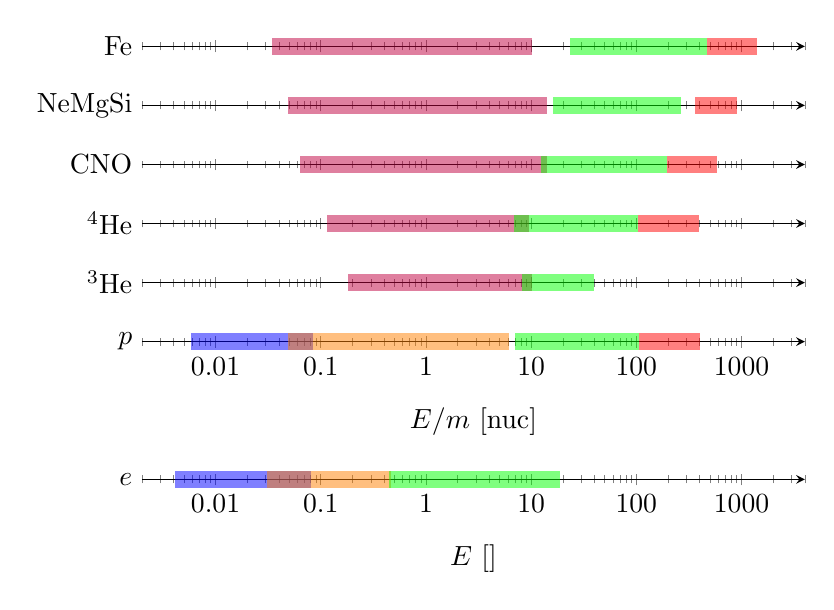
\begin{tikzpicture}
	\def\xmin{0.002}
	\def\xmax{4000}

	% EPT energy ranges, based on calibration as of 2020-10-01
	% ELECTRONS
	\begin{semilogxaxis}[xmin=\xmin, xmax=\xmax, axis x line=middle, hide y axis, ymin=-2,ymax=2,
					 height=2cm, width=10cm,
					 xlabel={$E$ [\si{\mega\electronvolt}]},
					 x label style={at={(axis description cs:0.5,-1.2)},anchor=north},clip=false,
					 log ticks with fixed point, x tick label style={/pgf/number format/1000 sep={}},yshift=0.25cm]
		\fill[blue, opacity=0.5] (axis cs:0.0041, -1) rectangle (axis cs:0.080, 1);
		\fill[orange, opacity=0.5] (axis cs:0.031, -1) rectangle (axis cs:0.47, 1);
		\fill[green, opacity=0.5] (axis cs:0.45, -1) rectangle (axis cs:18.8, 1);
		\node[left] at (axis cs:\xmin, 0) {$e$};
	\end{semilogxaxis}
	
	% PROTONS
	\begin{semilogxaxis}[xmin=\xmin, xmax=\xmax, axis x line=middle, hide y axis, ymin=-2,ymax=2,
	height=2cm, width=10cm, 
	xlabel={$E/m$ [\si{\mega\electronvolt\per nuc}]},
	x label style={at={(axis description cs:0.5,-1.2)},anchor=north},
	yshift=2cm, clip=false,
	log ticks with fixed point, x tick label style={/pgf/number format/1000 sep={}}]
		\fill[blue, opacity=0.5] (axis cs:0.0058, -1) rectangle (axis cs:0.085, 1);
		\fill[orange, opacity=0.5] (axis cs:0.049, -1) rectangle (axis cs:6.1, 1);
		\fill[green, opacity=0.5] (axis cs:7.0, -1) rectangle (axis cs:105, 1);
		\fill[red, opacity=0.5] (axis cs:105, -1) rectangle (axis cs:401.13, 1);
		%\fill[purple, opacity=0.5] (axis cs:0.24, 1) rectangle (axis cs:9.4, 3);
		\node[left] at (axis cs:\xmin, 0) {$p$};
	\end{semilogxaxis}
	
	% 3He
	\begin{semilogxaxis}[xmin=\xmin, xmax=\xmax, axis x line=middle, hide y axis, ymin=-2,ymax=2,
	height=2cm, width=10cm, xticklabels={,,},
	yshift=2.75cm, clip=false]
		\fill[purple, opacity=0.5] (axis cs:0.18, -1) rectangle (axis cs:10.2, 1);
		\fill[green, opacity=0.5] (axis cs:8.1, -1) rectangle (axis cs:39.7, 1);
		\node[left] at (axis cs:\xmin, 0) {$^3$He};
	\end{semilogxaxis}
	
	% 4He
	\begin{semilogxaxis}[xmin=\xmin, xmax=\xmax, axis x line=middle, hide y axis, ymin=-2,ymax=2,
	height=2cm, width=10cm, xticklabels={,,},
	yshift=3.5cm, clip=false]
		%\fill[orange, opacity=0.5] (axis cs:6.37, 1) rectangle (axis cs:24.51, 3);
		\fill[purple, opacity=0.5] (axis cs:0.115, -1) rectangle (axis cs:9.493, 1);
		\fill[green, opacity=0.5] (axis cs:6.877, -1) rectangle (axis cs:104, 1);
		\fill[red, opacity=0.5] (axis cs:104, -1) rectangle (axis cs:392.84, 1);
		\node[left] at (axis cs:\xmin, 0) {$^4$He};
	\end{semilogxaxis}
	
	% CNO
	\begin{semilogxaxis}[xmin=\xmin, xmax=\xmax, axis x line=middle, hide y axis, ymin=-2,ymax=2,
	height=2cm, width=10cm, xticklabels={,,},
	yshift=4.25cm, clip=false]
		\fill[purple, opacity=0.5] (axis cs:0.064, -1) rectangle (axis cs:14.13, 1);
		\fill[green, opacity=0.5] (axis cs:12.54, -1) rectangle (axis cs:197, 1);
		\fill[red, opacity=0.5] (axis cs:197, -1) rectangle (axis cs:578.37, 1);
		\node[left] at (axis cs:\xmin, 0) {CNO};
	\end{semilogxaxis}
	
	% NeMgSi
	\begin{semilogxaxis}[xmin=\xmin, xmax=\xmax, axis x line=middle, hide y axis, ymin=-2,ymax=2,
	height=2cm, width=10cm, xticklabels={,,},
	yshift=5cm, clip=false]
		\fill[purple, opacity=0.5] (axis cs:0.049, -1) rectangle (axis cs:14.13, 1);
		\fill[green, opacity=0.5] (axis cs:16.2, -1) rectangle (axis cs:268.42, 1);
		\fill[red, opacity=0.5] (axis cs:358, -1) rectangle (axis cs:915.03, 1);
		\node[left] at (axis cs:\xmin, 0) {NeMgSi};
	\end{semilogxaxis}
	
	% Fe
	\begin{semilogxaxis}[xmin=\xmin, xmax=\xmax, axis x line=middle, hide y axis, ymin=-2,ymax=2,
	height=2cm, width=10cm, xticklabels={,,},
	yshift=5.75cm, clip=false]
		\fill[purple, opacity=0.5] (axis cs:0.0346, -1) rectangle (axis cs:10.29, 1);
		\fill[green, opacity=0.5] (axis cs:23.66, -1) rectangle (axis cs:465.7, 1);
		\fill[red, opacity=0.5] (axis cs:465.8, -1) rectangle (axis cs:1388.40, 1);
		\node[left] at (axis cs:\xmin, 0) {Fe};
	\end{semilogxaxis}
\end{tikzpicture}
%\end{document}
	\caption[\acs{EPD} energy coverage]{Energy coverage of the different sensors in the \ac{EPD} suite for electrons and different ion species, based on the current science data products as of October 2020. This is an updated and enhanced version of Figure 3 from \citet{RodriguezPacheco-2019-EPD}. In the case of the CNO and NeMgSi groups, the responses for carbon and neon were taken as an example, the other species differ slightly. For simplicity, \acs{SIS} protons, \acs{EPT} stopping helium as well as \acs{EPT} penetrating data products are excluded from this plot. For the penetrating data products of \acs{HET}, the highest energy bin \citep[as given by][Appendix A]{Elftmann-2020-PhD} is not included, as its coverage extends to infinity.}
	\label{fig:epd_energy_ranges}
\end{figure}
The lowest energies of electrons and protons, slightly above the solar wind up to \SI{80}{\kilo\electronvolt}, are measured by the \ac{STEP} telescope, which is followed by the \ac{EPT} for medium energies up to $\sim\SI{6}{\mega\electronvolt}$ for protons and \SI{450}{\kilo\electronvolt} for electrons. Both \ac{EPT} and \ac{STEP} mainly measure electrons and protons and cannot separate heavy ion species, so they are supplemented with the \ac{SIS}, a time-of-flight based instrument that measures 12 ion species from H to Fe between \SI{14}{\kilo\electronvolt\per nuc} and \SI{20.5}{\mega\electronvolt\per nuc}. The highest energies of electrons and all ion species are covered by the \ac{HET}, whose measurements are, similarly to \ac{RAD}, based on the $\dd E/\dd x$-$E$ method.

The double-ended \ac{HET} sensor head is shown in Figure \ref{subfig:het-sensorhead-cad}. Two of these sensors are installed onboard the \ac{SolO} spacecraft on the side decks, which provide four viewing directions: Sunward, antisunward, north and south. The sunward and antisunward fields of view (HET 1) are pointed \SI{35}{\degree} away from the radial direction within the ecliptic, which corresponds to the mean direction of the nominal Parker spiral, while the north and south fields of view (HET 2) are pointed out of the ecliptic. The \ac{HET} telescopes each consist of four silicon solid-state detectors (A1, B1, B2, A2) and a Bi$_4$Ge$_3$O$_{12}$ (BGO) scintillator (C) in the center. This setup is similar to \ac{MSL} (\autoref{sec:mslrad}), though there is no second plastic scintillator for the detection of neutral particles.

\begin{figure}
	\centering
	\subfloat[\acs{CAD} rendering of the \ac{HET} sensor head. Taken from \citet{RodriguezPacheco-2019-EPD}, Fig. 31.]{
		\includegraphics[width=0.6\textwidth]{images/het.png}
		\label{subfig:het-sensorhead-cad}
	}\\
	\subfloat[Schematic diagram of the \ac{HET} sensor head. Exemplary particle trajectories ending up in different data products are shown by the arrows: \textcolor{red}{stopping in B}, \textcolor{green}{stopping in C}, \textcolor{blue}{penetrating}, \textcolor{Aquamarine}{GCR channel}, \textcolor{orange}{C single counter}.]{
		%\documentclass{standalone}
%\usepackage[dvipsnames]{xcolor}
%\usepackage{tikz}
%\usepackage{amsmath}
%\usepackage{siunitx}

%\usetikzlibrary{calc}
%\usetikzlibrary{decorations.pathmorphing}

%\definecolor{light-gray}{gray}{0.9}

%\begin{document}
\begin{tikzpicture}[scale=0.4]
    \tikzset{%
        add/.style args={#1 and #2}{
            to path={%
                ($(\tikztostart)!-#1!(\tikztotarget)$)--($(\tikztotarget)!-#2!(\tikztostart)$)%
                \tikztonodes},add/.default={.2 and .2}}
    }   
    
    \def\Sithickness{0.05}
    
    % A1
    \draw[fill=light-gray] (-\Sithickness, -0.87) rectangle (\Sithickness, 0.87) node[above,yshift=2mm]{\small A1};
    \draw (-\Sithickness, -0.4) -- (\Sithickness, -0.4);
    \draw (-\Sithickness, 0.4) -- (\Sithickness, 0.4);
    
    % B1
    \draw[fill=light-gray] (4.4-\Sithickness, -1.82) rectangle (4.4+\Sithickness, 1.82) node[above]{\small B1};
    \draw (4.4-\Sithickness, -0.4) -- (4.4+\Sithickness, -0.4);
    \draw (4.4-\Sithickness, 0.4) -- (4.4+\Sithickness, 0.4);
    \draw (4.4-\Sithickness, -0.87) -- (4.4+\Sithickness, -0.87);
    \draw (4.4-\Sithickness, 0.87) -- (4.4+\Sithickness, 0.87);
    
    % C
    \draw[fill=light-gray] (4.635, -1.75) rectangle ++(2, 3.5);
    \node[above, yshift=0.5mm] at (5.635, 1.75) {\small C};
    
    % B2
    \draw[fill=light-gray] (6.9-\Sithickness, -1.82) rectangle (6.9+\Sithickness, 1.82) node[above]{\small B2};
    \draw (6.9-\Sithickness, -0.4) -- (6.9+\Sithickness, -0.4);
    \draw (6.9-\Sithickness, 0.4) -- (6.9+\Sithickness, 0.4);
    \draw (6.9-\Sithickness, -0.87) -- (6.9+\Sithickness, -0.87);
    \draw (6.9-\Sithickness, 0.87) -- (6.9+\Sithickness, 0.87);
    
    % A2
    \draw[fill=light-gray] (11.3-\Sithickness, -0.87) rectangle (11.3+\Sithickness, 0.87) node[above,yshift=2mm]{\small A2};
    \draw (11.3-\Sithickness, -0.4) -- (11.3+\Sithickness, -0.4);
    \draw (11.3-\Sithickness, 0.4) -- (11.3+\Sithickness, 0.4);
    
    % FOV
    \draw[add=0.1 and 0, dashed, opacity=0.5] (0, -0.87) to (6.9, 1.82);
    \draw[add=0.1 and 0, dashed, opacity=0.5] (0, 0.87) to (6.9, -1.82);
    \draw[add=0.1 and 0, dashed, opacity=0.5] (11.3, -0.87) to (4.4, 1.82);
    \draw[add=0.1 and 0, dashed, opacity=0.5] (11.3, 0.87) to (4.4, -1.82);
    
    \draw[|<->|] (0, 0.87) ++ (180-21.45:0.5) arc (180-21.45:180+21.45:2.4+0.48) node[midway, left] {\small\SI{42.9}{\degree}};
    

    \draw[thick, red, -latex] (-0.2, 0.2) -- (4.4, 0.5);
    \draw[thick, green, -latex] (-0.2, 0) -- (5.7, 0.1);
    \draw[thick, blue, -latex] (-0.2, -0.2) -- (11.5, -0.5);
    \uncover<2->{
        \draw[thick, Aquamarine, -latex] (2.5, 2) -- (8.4, -2);
        \draw[thick, orange, -latex] (5.635, -2.3) -- (5.635, -1);
    }
\end{tikzpicture}
%\end{document}
		\label{subfig:het-sensorhead-diagram}
	}
	\caption[\acs{HET} sensor head]{\acs{HET} sensor head}
	\label{fig:het-sensorhead}
\end{figure}

Charged particles that enter through one of the A detectors and then stop in B or C are measured in the \ac{HET} data products for stopping particles, which are defined using the ABnC and ABC coincidence conditions (as shown in red and green in \autoref{subfig:het-sensorhead-diagram}). These particles are fully analyzed using the $\dd E/\dd x$-$E$ method, i.e. their primary energy and charge can be directly determined.
Ions with higher energies (e.g. $\gtrsim\SI{100}{\mega\electronvolt\per nuc}$ for protons and helium) penetrate the whole telescope (ABCBA coincidence, shown in blue in \autoref{subfig:het-sensorhead-diagram}). In this case, as with the penetrating particles in \ac{RAD}, the particles are not fully analyzed, but up to a few \SI{100}{\mega\electronvolt}, the particle direction and primary energy can still be estimated based on the different \ac{LET} at each end of the telescope (e.g. in the A1 and A2 detectors).

Similarly to \ac{RAD}, these energy-resolved data products are very useful for \ac{SEP} events as well as to calculate longterm \ac{GCR} spectra, but they do not have high enough count rates to study short-term variations of the \ac{GCR}. Alternatively, \ac{HET} also produces a data product using the BCB coincidence (irrespective of the A detectors, shown in turquoise in \autoref{subfig:het-sensorhead-diagram}), which significantly increases the opening angle at the cost of lower energy and species resolution. In addition, basic single detector count rates (level 1 trigger rates) without any coincidence conditions applied are available in \ac{HET}'s housekeeping data, and the count rates for the C detector are best suited for measuring short-term variations due to its large volume. The response function of this single detector counter is derived in \autoref{chp:HETSimulation}.

Further details about the design of the \ac{HET} instrument, the definition of its data products and their calibration can be found in \citet{Elftmann-2020-PhD}. 

\section{Neutron monitor measurements}
\label{sec:neutronmonitors}

First developed in the 1950s \citep[see e.g.][]{Simpson-2000}, ground-based neutron monitors have historically been the most widely available instrument for the measurement of the cosmic ray flux at Earth. Neutron monitors measure secondary neutrons generated by the primary \ac{GCR} and \ac{SEP} particles in the Earth's atmosphere. Neutron monitors are typically large and heavy instruments, as they need one or more large tubes of lead to have a sufficiently high efficiency for detecting high-energy neutrons. Such devices have been deployed at numerous locations around the globe, and many of them have been producing measurements almost continuously for multiple decades. Today, data from the global network of more than 50 neutron monitors \citep[e.g.][]{Moraal-2000} are archived at the Neutron Monitor Database (NMDB)\footnote{\url{https://www.nmdb.eu}}, and many of these stations are also providing realtime data.

Similar to \ac{RAD} on Mars (\autoref{sec:mslrad}), neutron monitor measurements are influenced by the Earth's atmosphere, as well as the magnetosphere, and thus any cosmic ray particle needs a certain minimum energy to be able to create a secondary neutron in the atmosphere that reaches the ground and can be detected in a neutron monitor.

% TODO: atmospheric and magnetic cutoff

The cutoff energy is often also expressed in terms of a rigidity
\begin{equation}
	R = \frac{pc}{q}
\end{equation}
which is given in units of \si{V}. $p$ is the particle's momentum, $q$ its charge and $c$ the speed of light. The benefit of using rigidity instead of (kinetic) energy is that the same rigidity results in the same trajectory in a magnetic field independent of the particle species. Using relativistic relations, $R$ can be rewritten in terms of the particle's charge $e$, rest mass $m_0$ and kinetic energy $E_\text{kin}$ as:
\begin{equation}
    R = \frac{1}{Ze} \sqrt{E_\text{kin}(E_\text{kin} + 2 m_0 c^2)}
\end{equation}
\citep[see e.g.][for the detailed derivation]{Moraal-2013}, and this approaches $R \approx E_\text{kin}/Ze$ for highly relativistic particles ($E_\text{kin}\gg m_0 c^2$). So, for example, a \SI{100}{\giga\electronvolt} proton ($Z=1$) has a rigidity of approximately \SI{100}{\giga\volt}.

% TODO: South pole neutron monitor, GSM.

\section{The STEREO Heliospheric Imagers}
\label{sec:stereohi}

\begin{figure}
    \centering
    \includegraphics[width=0.8\linewidth]{images/secchi_fov}
    \caption[Fields of view of the \acs{STEREO} SECCHI telescopes]{Fields of view of the \ac{STEREO} SECCHI telescopes EUVI, COR1, COR2 (circles on the right side), and HI1 and HI2. Source: NASA/STEREO/GSFC}
    \label{fig:secchifov}
\end{figure}
